\lab{Optimal Reentry of a Spacecraft}{Optimal Reentry of a Spacecraft}
\label{lab:reentry}
\objective{ We consider the problem of minimizing the heating experienced by a spacecraft during reentry. 
The boundary value problem (BVP) associated with the reentry of a spacecraft is inherently challenging: the craft must descend quickly enough to enter the atmosphere, but pull out soon enough to prevent overheating or crashing. 
Problems involving variational calculus and optimal control often include the numerical solution of a challenging BVP. }

\begin{figure}
\centering
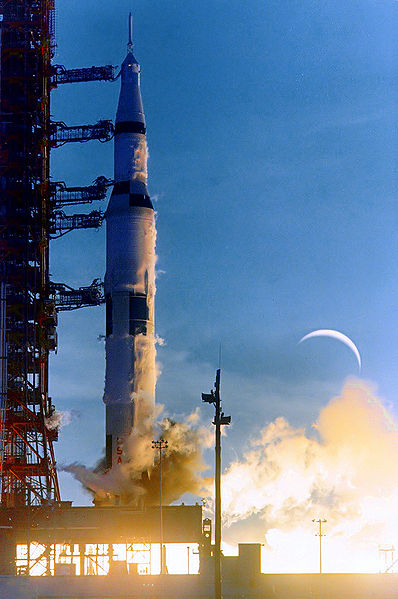
\includegraphics[width=6cm]{Apollo8_during_Launch.jpg}
\caption{Apollo 8 during launch}
\label{fig:reentry:apollo8}
\end{figure}

A fundamental topic considered in aerospace engineering is the process of landing a spacecraft. 
Landing a spacecraft requires a massive reduction in the kinetic energy of the craft. 
That reduction can be accomplished either through the use of massive quantities of fuel (very expensive), or by  transforming kinetic energy into heat. 
That heat must then be absorbed by the atmosphere and the spacecraft. 
The question then is how to choose the optimal path for reentry into the atmosphere, where the total heating experienced by the craft is minimized. 


We begin by giving a control system\footnote{This control problem and its numerical solution are thoroughly described in `Introduction to Numerical Analysis' by J. Stoer, R. Bulirsch (pg 524). 
We will mirror their presentation throughout this lab.}
describing the path of a spacecraft through the atmosphere 
(we assume the spacecraft is similar to the Apollo craft).
Our dependent variables to consider are the velocity $v$ of the spacecraft,  the angle $\gamma$ of the flight path, and the normalized altitude $\xi$ above the Earth's surface. ($\xi = h/R$, where $R$ is the radius of the Earth and $h$ the altitude of the spacecraft above the Earth.) 
A control variable  $u$ will be used to represent the angle of attack of the spacecraft. 
The flight path can then be described by 
\begin{align}
\begin{split}
\dot{v} &= -s\rho v^2C_D(u) - \frac{g\sin(\gamma)}{(1+\xi)^2},\\
\dot{\gamma} &= s \rho v C_L(u) + \frac{v \cos(\gamma)}{R(1+\xi)} - \frac{g \cos \gamma}{v(1+\xi)^2},\\
\dot{\xi} &= \frac{v \sin \gamma}{R}.
\end{split} \label{eqn:reentry:control_system}
\end{align}
$C_D$ and $C_L$ represent drag and lift coefficients, and are functions of $u$: $C_D(u) = 1.174 - .9\cos u$, $C_L(u) = 0.6\sin u$. 
The atmospheric density $\rho$ is a function of height, which we represent by $\rho(\xi) = \rho_0e^{-R\beta\xi}$, where  $\rho_0$ is the atmospheric density at the surface of the earth. 
Other parameters include the force of gravity $g$, and $s = \frac{1}{2}S/m$, where $S$ is the frontal area of the craft and $m$ is its mass.
The numerical values we will use are coded below, along with the drag and lift functions. 
\begin{lstlisting}
from math import sin, cos, exp

from numpy import array
from scipy.special import erf
from scikits import bvp_solver

R = 209
beta = 4.26
rho0 = 2.704e-3
g = 3.2172e-4
s = 26600 

def C_d(u): 
	return 1.174 - 0.9*cos(u)

def C_l(u): 
	return 0.6*sin(u)
\end{lstlisting}
% $g = 3.2172\times10^{-4}$, $s = 26,600$, $R = 209$ $(209\times 10^5 \text{ ft})$, $\beta = 4.26$ and $\rho_0 = 2.704\times 10^{-3}$.

We will require that the trajectory of the spacecraft satisfy the boundary conditions
\begin{equation}
  \begin{split}
    v(0) &= 0.36 \quad (36000 \text{ ft/sec})\\
    \gamma(0) &= -8.1^\circ \frac{\pi}{180^\circ}\\
    \xi(0)&= \frac{4}{R}\quad (h = 400000 \text{ ft})
  \end{split} 
\quad \quad \quad \quad \quad
  \begin{split}
    v(T) &= 0.27\\
    \gamma(T) &= 0 \\
	\xi(T)&= \frac{2.5}{R}
  \end{split} \label{eqn:reentry:BCs}
\end{equation}
where $T$ represents the time at the end of the (first) reentry maneuver. 
These boundary conditions are similar to those encountered at the end of each Apollo mission to the moon. 


To simpify notation, we will also write \eqref{eqn:reentry:control_system} in the form $y' = G(y)$, where $y = [y_0, y_1, y_2]^T=[v,\gamma, \xi]^T$ and $G$ has component functions $G = [G_0, G_1, G_2]^T$. 
% \begin{align}
% \begin{split}
% 	v(0) &= 0.36 \quad (36000 \text{ ft/sec}),\\
% 	\gamma(0) &= -8.1^\circ \frac{\pi}{180^\circ}, \\
% 	\xi(0)&= \frac{4}{R}\quad (h = 400000 \text{ ft}), \\
% 	v(T) &= 0.27,\\
% 	\gamma(T) &= 0, \\
% 	\xi(T)&= \frac{2.5}{R}, \\
% \end{split}
% \end{align}
%
The total heating is 
\[
J[u] = \int_0^T 10y_0^3 \sqrt{\rho}.
\]
The Hamiltonian corresponding to this control system is 
\begin{align}
H &=  10y_0^3 \sqrt{\rho} + \lambda_0G_0 + \lambda_1G_1 + \lambda_2G_2,
\end{align}
where $\lambda = [\lambda_0,\lambda_1,\lambda_2]^T$ is the adjoint variable. 
The optimal state and adjoint equations are thus given by 
\begin{align}
\begin{split}
	\dot{y} &= H_{\lambda},\\
	\dot{\lambda} &= -H_{y} \label{eqn:reentry:full_system}
\end{split}
\end{align}
To our boundary conditions we add the terminal condition that $H = 0$ at $t = T$. 
Finally, from the condition $\frac{\partial H}{\partial u} = 0$ we find that the optimal control satisfies 
\begin{align}
\tan u &= \frac{6\lambda_1}{9y_0\lambda_0}.
\end{align}

Most BVP solvers require an equal number of differential equations and boundary conditions. 
Currently we have a free boundary value problem; there are 6 ODEs and 7 boundary conditions, and the length of the reentry maneuver, $T$, is still unknown. 
By making the transformation $x = t/T$, and treating $T$ as a dependent variable, the BVP is now defined on the interval $(0,1)$ and is augmented with an additional ODE: 
\begin{align}
\begin{split}
	y' &= TH_{\lambda},\quad ' = \frac{d}{dx},\\
	\lambda' &= -TH_{y},\\
	T' &= 0. \label{eqn:reentry:full_system}
\end{split}	
\end{align}
This BVP has 7 ODEs, and with the 7 boundary conditions introduced earlier it has the required form.
% \footnote{BNDSCO - A program for the numerical solution of optimal control problems, H.J. Oberle and W. Grimm, 1989}

\begin{problem}
	Write a function \li{ode} that implements the ODEs for the original control system along with the adjoint equations \eqref{eqn:reentry:full_system}. 
\begin{lstlisting}
def ode(x,y):
	# Parameters:
	# x: independent variable (unused in our ODEs)
	# y: vector-valued dependent variable; it is an ndarray 
	# 	 with shape (7,)
	
	# Returns: 
	# ndarray of length (7,) that evalutes the RHS of the ODES
\end{lstlisting}
\end{problem}



\begin{figure}
\centering
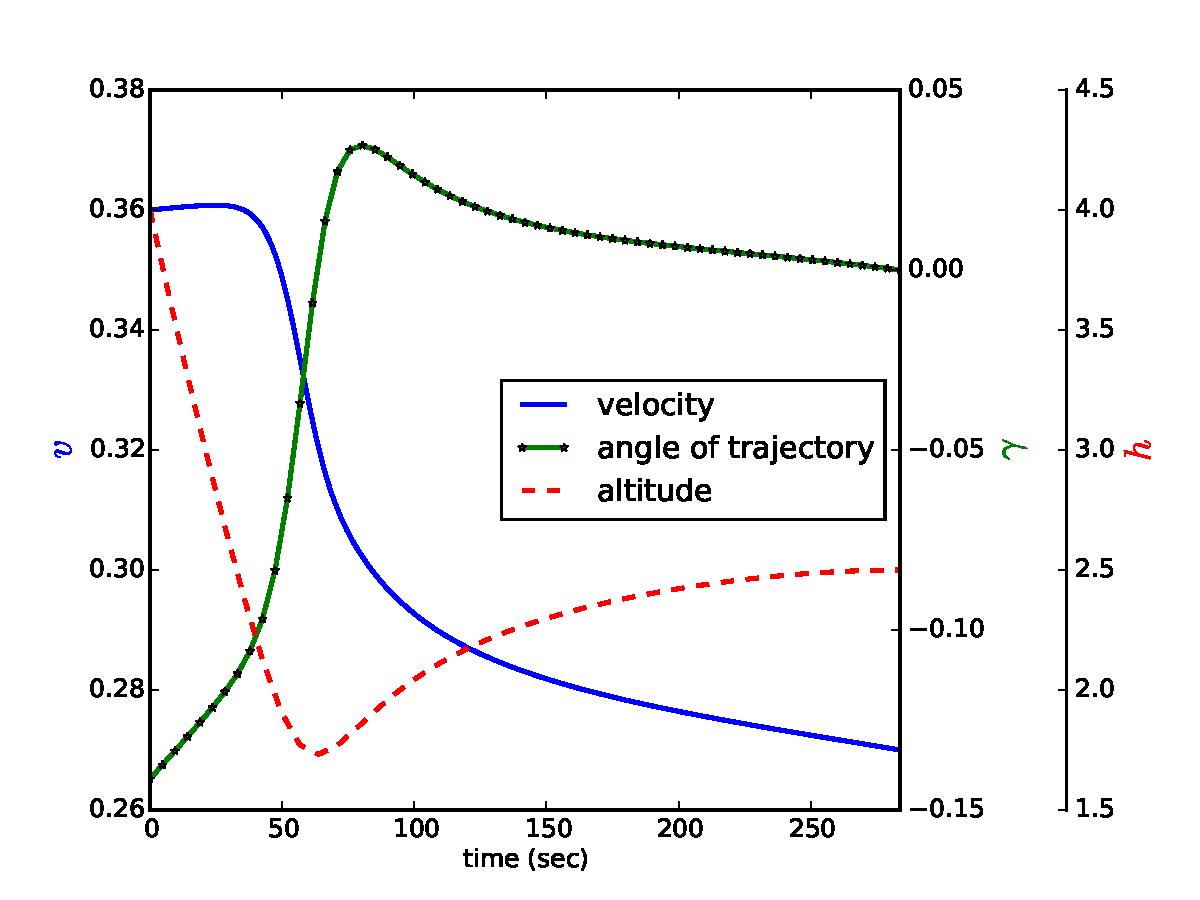
\includegraphics[width=\textwidth]{solutions.pdf}
\caption{The optimal path for the reentry maneuver of a spacecraft. This path minimizes the heating of the spacecraft, and satisfies  \eqref{eqn:reentry:full_system},\eqref{eqn:reentry:BCs}, and the terminal condition $H(T) = 0$.
}
\label{fig:reentry:solutions}
\end{figure}



\section*{Constructing an Initial Guess}
We will use the BVP solver \li{scikits.bvp_solver}. 
Like any solver capable of handling nonlinear problems, \li{bvp_solver} requires an initial guess to jump-start its Newton-like iteration process. 
Our nonlinear BVP is very sensitive, and requires an initial guess that is quite close to the solution.  
This sensitivity is physically meaningful. The spacecraft is traveling at a speed far greater than a typical aircraft. If the control is not aggressive, the spacecraft will fall/`bounce' back into space as it encounters the atmosphere at a high velocity. 
However, if the control lasts too long, the craft will overheat or crash.

Since this is a sensitive problem, we will use a heuristic method to  construct a good initial guess.
From aerospace engineers we know that the control $u$ should empirically look like Figure \ref{fig:reentry:estimate_u}; 
we can create a smooth approximation of the form $u = p_0\erf(p_1(p_2-t/T))$, where $p_0, p_1,$ and $p_2$ are unknown constants. 
To help us determine these constants, and to find good initial guesses for $v, \gamma$, and $\xi$, we define an auxiliary BVP to help us come up with a good initial guess for the original BVP:
\begin{align}
\begin{split}
\dot{y_0} &= -s\rho y_0^2C_D(u) - \frac{g\sin(y_1)}{(1+y_2)^2},\\
\dot{y_1} &= s \rho y_0 C_L(u) + \frac{y_0 \cos(y_1)}{R(1+y_2)} - \frac{g \cos y_1}{y_0(1+y_2)^2},\\
\dot{y_2} &= \frac{y_0 \sin y_1}{R} ,\\
\dot{p_0} &= 0, \\
\dot{p_1} &= 0, \\
\dot{p_2} &= 0.
\end{split} \label{eqn:reentry:control_system_auxiliary}
\end{align}

This auxiliary BVP is defined on the interval $[0,T]$, where $T$ is unknown. 
We guess at $T$: the maneuver will occur quickly, so how about 230 seconds?
Below we create functions for the ODE and for the boundary conditions. 
\begin{lstlisting}
T0 = 230.

def ode_auxiliary(x,y):
	u = y[3]*erf( y[4]*(y[5]-x/T0) )
	rho = rho0*exp(-beta*R*y[2])
	out = array([-s*rho*y[0]**2*C_d(u) - g*sin(y[1])/(1+y[2])**2,
				  ( s*rho*y[0]*C_l(u) + y[0]*cos(y[1])/(R*(1 + y[2])) - 
				  g*cos(y[1])/(y[0]*(1+y[2])**2) ),
				  y[0]*sin(y[1])/R,
				  0,
				  0,
				  0		])
	return out
	
def bcs_auxiliary(ya,yb):
	# If the problem is defined on the interval [a,b], ya = y(a) and yb = y(b), 
	# ya[0] = y_0(a), etc.
	# bvp_solver will attempt to make each of the entries below zero in the 
	# numerical solution.
	
	out1 = array([ya[0]-.36,
				  ya[1]+8.1*pi/180,
				  ya[2]-4/R
				  ])
	out2 = array([yb[0]-.27,
				  yb[1],
				  yb[2]-2.5/R
				  ])
	return out1, out2
\end{lstlisting}

The two main methods used by \li{bvp_solver} are \li{ProblemDefinition} and \li{solve}. You will want to look at their docstrings to learn more about their functionality. \li{solve} requires an initial guess, which you will create in Problem \ref{prob:reentry:guess}.
\begin{lstlisting}
problem_auxiliary = bvp_solver.ProblemDefinition(num_ODE = 6,
										  num_parameters = 0,
										  num_left_boundary_conditions = 3,
										  boundary_points = (0., T0),
										  function = ode_auxiliary,
										  boundary_conditions = bcs_auxiliary)
									
solution_auxiliary = bvp_solver.solve(problem_auxiliary,
									  solution_guess = guess_auxiliary)
								
N = 240 # Number of subintervals
x_array = linspace(0,T0,N+1)
y_array = solution_auxiliary(x_array)
	
\end{lstlisting}

\begin{figure}
\begin{minipage}[b]{.47\linewidth}
\centering
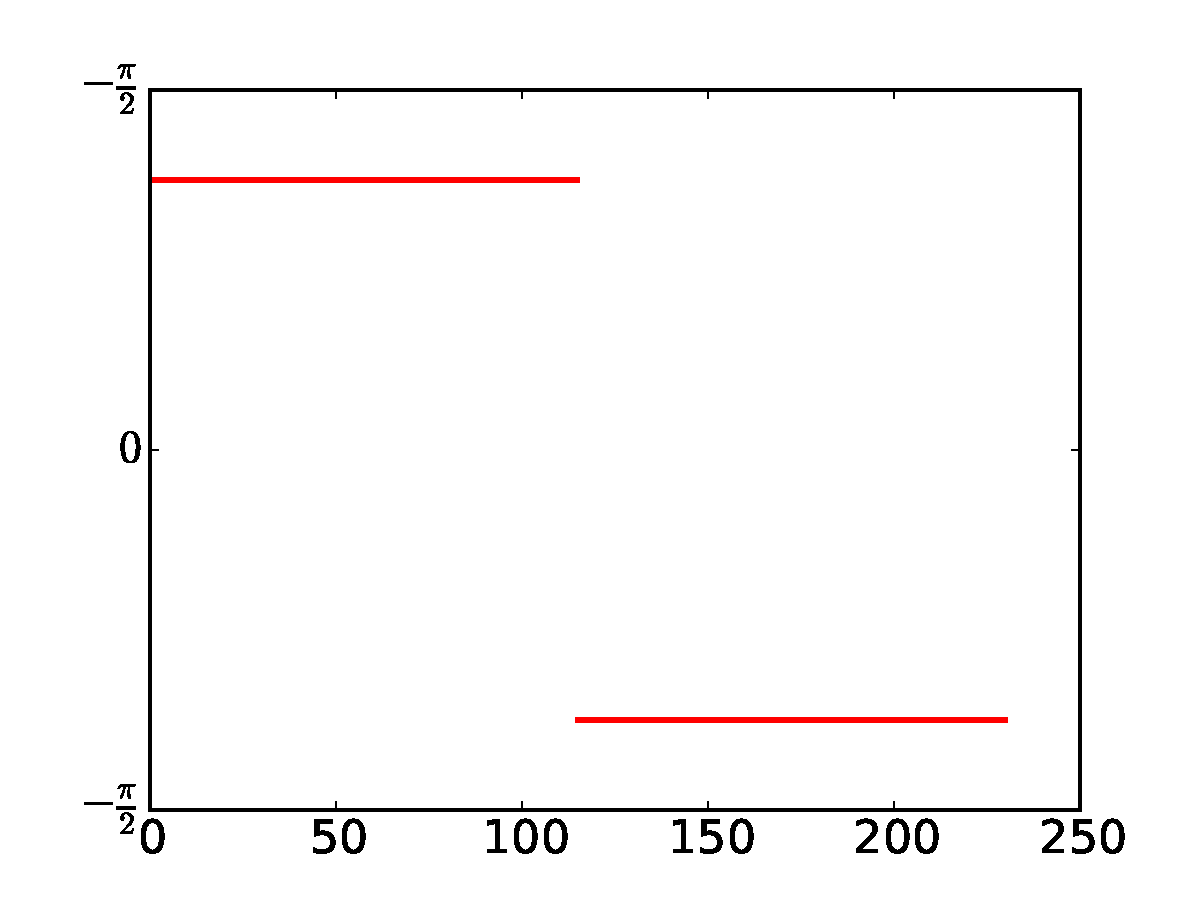
\includegraphics[width=\textwidth]{u_heuristic.pdf}
\caption*{Heuristic for the control $u$, provided by engineers. }
\end{minipage}
\hspace{0.5cm}
\begin{minipage}[b]{0.47\linewidth}
\centering
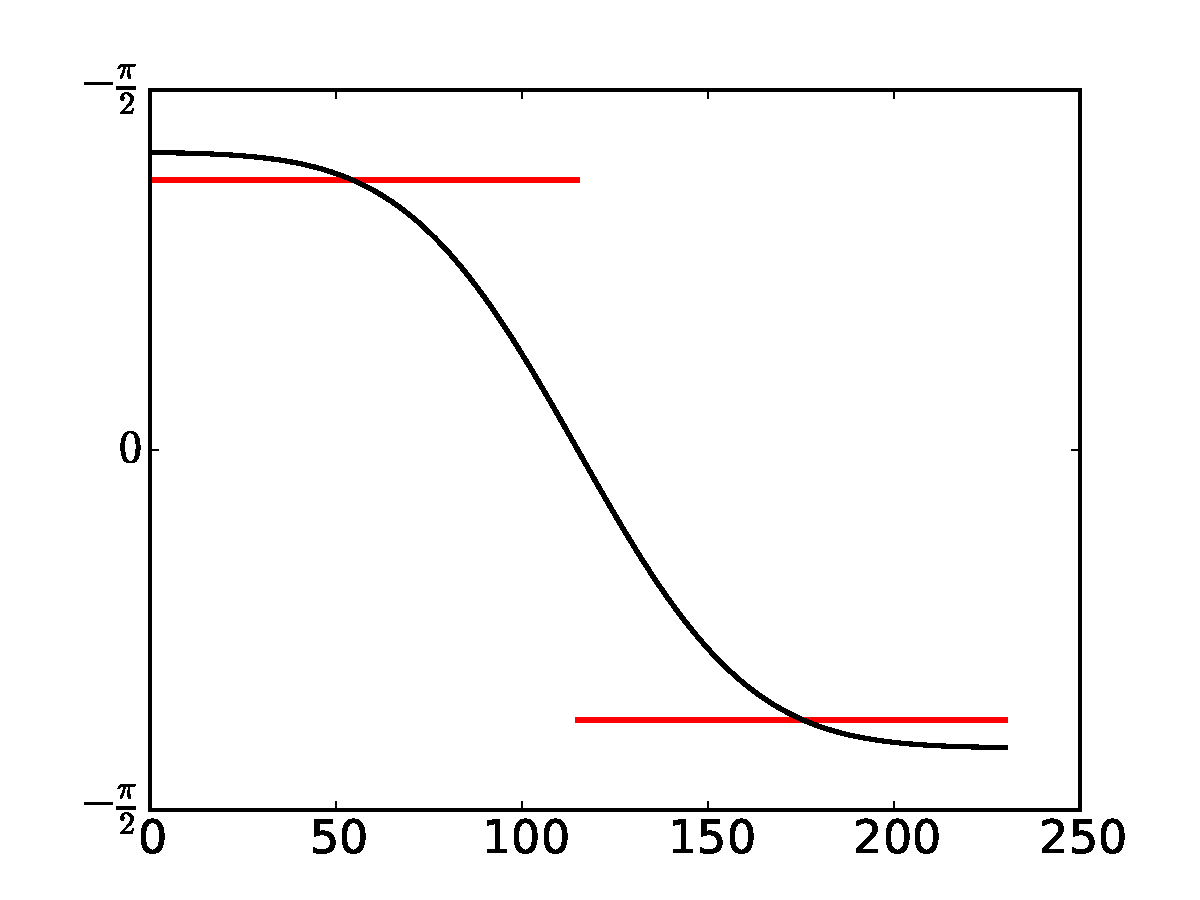
\includegraphics[width=\textwidth]{u_heuristic_smooth.pdf}
\caption*{A smooth initial approximation of the control.}
\end{minipage}
\caption{We construct a smooth estimate for the control $u$, by supposing the control has the form 
$u = p_0\erf(p_1(p_2-t/T))$ and estimating parameters $p_0, p_1, p_2$.}
\label{fig:reentry:estimate_u}
\end{figure}


\begin{problem}
	Write the function \li{guess_auxiliary} referenced in the code above. 
	This function provides an initial guess to \li{bvp_solver} for the auxiliary BVP described by  \eqref{eqn:reentry:control_system_auxiliary} and \eqref{eqn:reentry:BCs}.
	Use the heuristic data provided in Figure \ref{fig:reentry:estimate_u} to find good estimates of $p_0, p_1,$ and $p_2$. 
	Use Figure \ref{fig:reentry:solutions} to estimate the trajectories of $y_0, y_1,$ and $y_2$.
	Then run the code above to check that your initial guess is adequate. 
	\label{prob:reentry:guess}
\end{problem}






\begin{problem}
Incorporate this change into the function \li{ode} written earlier. 
Also write a function \li{bcs} that implements the full set of boundary conditions. 
\end{problem}

Discuss how to construct an initial guess for the original BVP. Specifically, how should the adjoint variables be estimated?
\begin{problem}
	Adapt your previous code to solve the original, dimension seven BVP. 
	Plot the control $u$. How long does the reentry maneuver take? 
\end{problem}


% \begin{figure}
% \begin{minipage}[b]{.47\linewidth}
% \centering
% 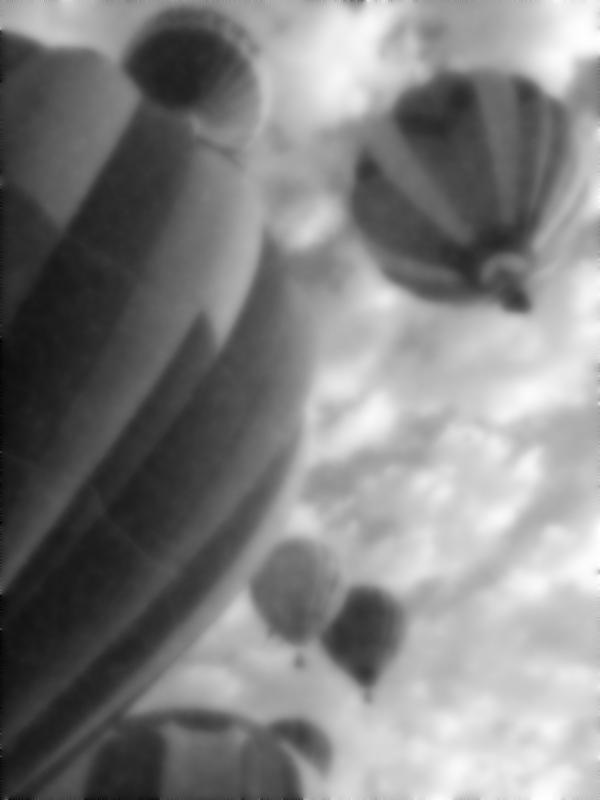
\includegraphics[width=\textwidth]{diffusion_denoised_baloons_resized_bw.jpg}
% \caption*{Initial diffusion-based approach}
% \end{minipage}
% \hspace{0.5cm}
% \begin{minipage}[b]{0.47\linewidth}
% \centering
% 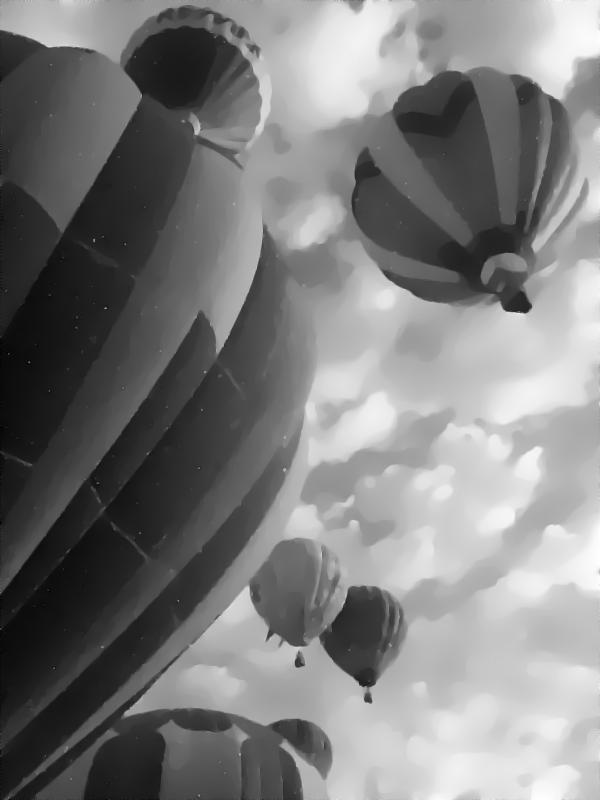
\includegraphics[width=\textwidth]{tv_denoised_baloons_resized_bw.jpg}
% \caption*{Total variation based approach}
% \end{minipage}
% \caption{The solutions of \eqref{tv_images:diffusion_flow} and \eqref{tv_images:tv_flow}, found using a first order Euler step in time and centered differences in space.}
% \label{fig:noise_compare_attempts}
% \end{figure}



% \begin{align}
% \begin{split}
% \end{split} \label{reentry:label}
% \end{align}
%
%
% \begin{problem}
%
% \begin{lstlisting}
% \end{lstlisting}
% \end{problem}


% \begin{figure}
% \centering
% 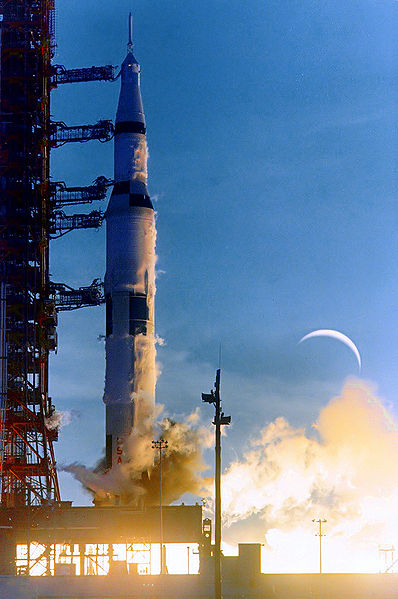
\includegraphics[width=6cm]{Apollo8_during_Launch.jpg}
% \caption{The Apollo 8 during launch}
% \label{fig:reentry:apollo8}
% \end{figure}







